\documentclass[11pt,twoside]{article}

%packages
\usepackage{geometry}                
\usepackage{graphicx,float}
\usepackage{amssymb,amssymb,amsmath,amsthm}
\usepackage{epstopdf}
\usepackage{natbib}
\usepackage{fancyhdr}
\usepackage{setspace}
\usepackage{extramarks}
\usepackage[usenames,dvipsnames]{color}
\usepackage{ifthen}
\usepackage{listings}
\usepackage[numbers]{natbib}
\usepackage{url}


%options
\DeclareGraphicsRule{.tif}{png}{.png}{`convert #1 `dirname #1`/`basename #1 .tif`.png}
\geometry{letterpaper}                   
\definecolor{MyDarkGreen}{rgb}{0.0,0.4,0.0}
\lstloadlanguages{Matlab}%
\lstset{language=Matlab,
        frame=single,
        basicstyle=\small\ttfamily,
        keywordstyle=[1]\color{Blue}\bf,
        keywordstyle=[2]\color{Purple},
        keywordstyle=[3]\color{Blue}\underbar,
        identifierstyle=,
        commentstyle=\usefont{T1}{pcr}{m}{sl}\color{MyDarkGreen}\small,
        stringstyle=\color{Purple},
        showstringspaces=false,
        tabsize=5,
        % Put standard MATLAB functions not included in the default
        % language here
        morekeywords={xlim,ylim,var,alpha,factorial,poissrnd,normpdf,normcdf},
        % Put MATLAB function parameters here
        morekeywords=[2]{on, off, interp},
        % Put user defined functions here
        morekeywords=[3]{FindESS},
        morecomment=[l][\color{Blue}]{...},
        numbers=left,
        firstnumber=1,
        numberstyle=\tiny\color{Blue},
        stepnumber=5,
	xleftmargin= -24mm,
        linewidth=160mm,
	postbreak=\space, breakindent=5pt, breaklines
	}

%footer and header
\newcommand{\reportTitle}{Axelrod’s Tournament with Noise}
\pagestyle{fancy}   
\fancyhead{} % clear all header fields
\fancyhead[LE,RO]{ \rightmark}
\fancyhead[LO,RE]{ \leftmark} 
\fancyfoot{}
\fancyfoot[LO,RE]{\reportTitle}                                                      
\fancyfoot[LE,RO]{\thepage}                
 \renewcommand\headrulewidth{0.4pt}                                    
 \renewcommand\footrulewidth{0.4pt}

% Includes a figure
% The first parameter is the label, which is also the name of the figure
%   with or without the extension (e.g., .eps, .fig, .png, .gif, etc.)
%   IF NO EXTENSION IS GIVEN, LaTeX will look for the most appropriate one.
%   This means that if a DVI (or PS) is being produced, it will look for
%   an eps. If a PDF is being produced, it will look for nearly anything
%   else (gif, jpg, png, et cetera). Because of this, when I generate figures
%   I typically generate an eps and a png to allow me the most flexibility
%   when rendering my document.
% The second parameter is the width of the figure normalized to column width
%   (e.g. 0.5 for half a column, 0.75 for 75% of the column)
% The third parameter is the caption.
\newcommand{\scalefig}[3]{
  \begin{figure}[ht!]
    % Requires \usepackage{graphicx}
    \centering
    \includegraphics[width=#2\columnwidth]{#1}
    %%% I think \captionwidth (see above) can go away as long as
    %%% \centering is above
    %\captionwidth{#2\columnwidth}%
    \caption{#3}
    \label{#1}
  \end{figure}}

% Includes a MATLAB script.
% The first parameter is the label, which also is the name of the script
%   without the .m.
% The second parameter is the optional caption.
\newcommand{\matlabscript}[2]
  {\begin{itemize}\item[]\lstinputlisting[caption=#2,label=#1]{#1.m}\end{itemize}}

% The environment takes two arguments, and will indent the left and right margins, respectively, 
% by the parameters’ values. Negative values will cause the margins to be narrowed, so 
% \begin{changemargin}{-1cm}{-1cm} narrows the left and right margins by 1 centimetre.                                     


\begin{document}



\thispagestyle{empty}

\begin{center}

\includegraphics[width=5cm]{ETHlogo.eps}

\bigskip


\bigskip


\bigskip


\LARGE{ 	Lecture with Computer Exercises:\\ }
\LARGE{ Modelling and Simulating Social Systems with MATLAB\\}

\bigskip

\bigskip

\small{Project Report}\\

\bigskip

\bigskip

\bigskip

\bigskip


\begin{tabular}{|c|}
\hline
\\
\textbf{\LARGE{Insert Title Here}}\\
\textbf{\LARGE{...}}\\
\\
\hline
\end{tabular}
\bigskip

\bigskip

\bigskip

\LARGE{Name 1 \& Name 2}



\bigskip

\bigskip

\bigskip

\bigskip

\bigskip

\bigskip

\bigskip

\bigskip

Zurich\\
May 2008\\

\end{center}



\newpage

%%%%%%%%%%%%%%%%%%%%%%%%%%%%%%%%%%%%%%%%%%%%%%%%%

\newpage
 \pagenumbering{Roman}
\section*{Agreement for free download}
\bigskip

\bigskip

\large We hereby agree to make our source code for this project freely available for download from the web pages of the SOMS chair. Furthermore, we assure that all source code is written by ourselves and is not violating any copyright restrictions.

\begin{center}
\bigskip\bigskip\bigskip\bigskip\bigskip\bigskip\bigskip\bigskip\bigskip


\large Andermatt Samuel
\bigskip\bigskip\bigskip\bigskip\bigskip\bigskip\bigskip\bigskip\bigskip

\large B\"osser Jonathan
\bigskip\bigskip\bigskip\bigskip\bigskip\bigskip\bigskip\bigskip\bigskip

\large Meier David

\end{center}
\newpage

%%%%%%%%%%%%%%%%%%%%%%%%%%%%%%%%%%%%%%%

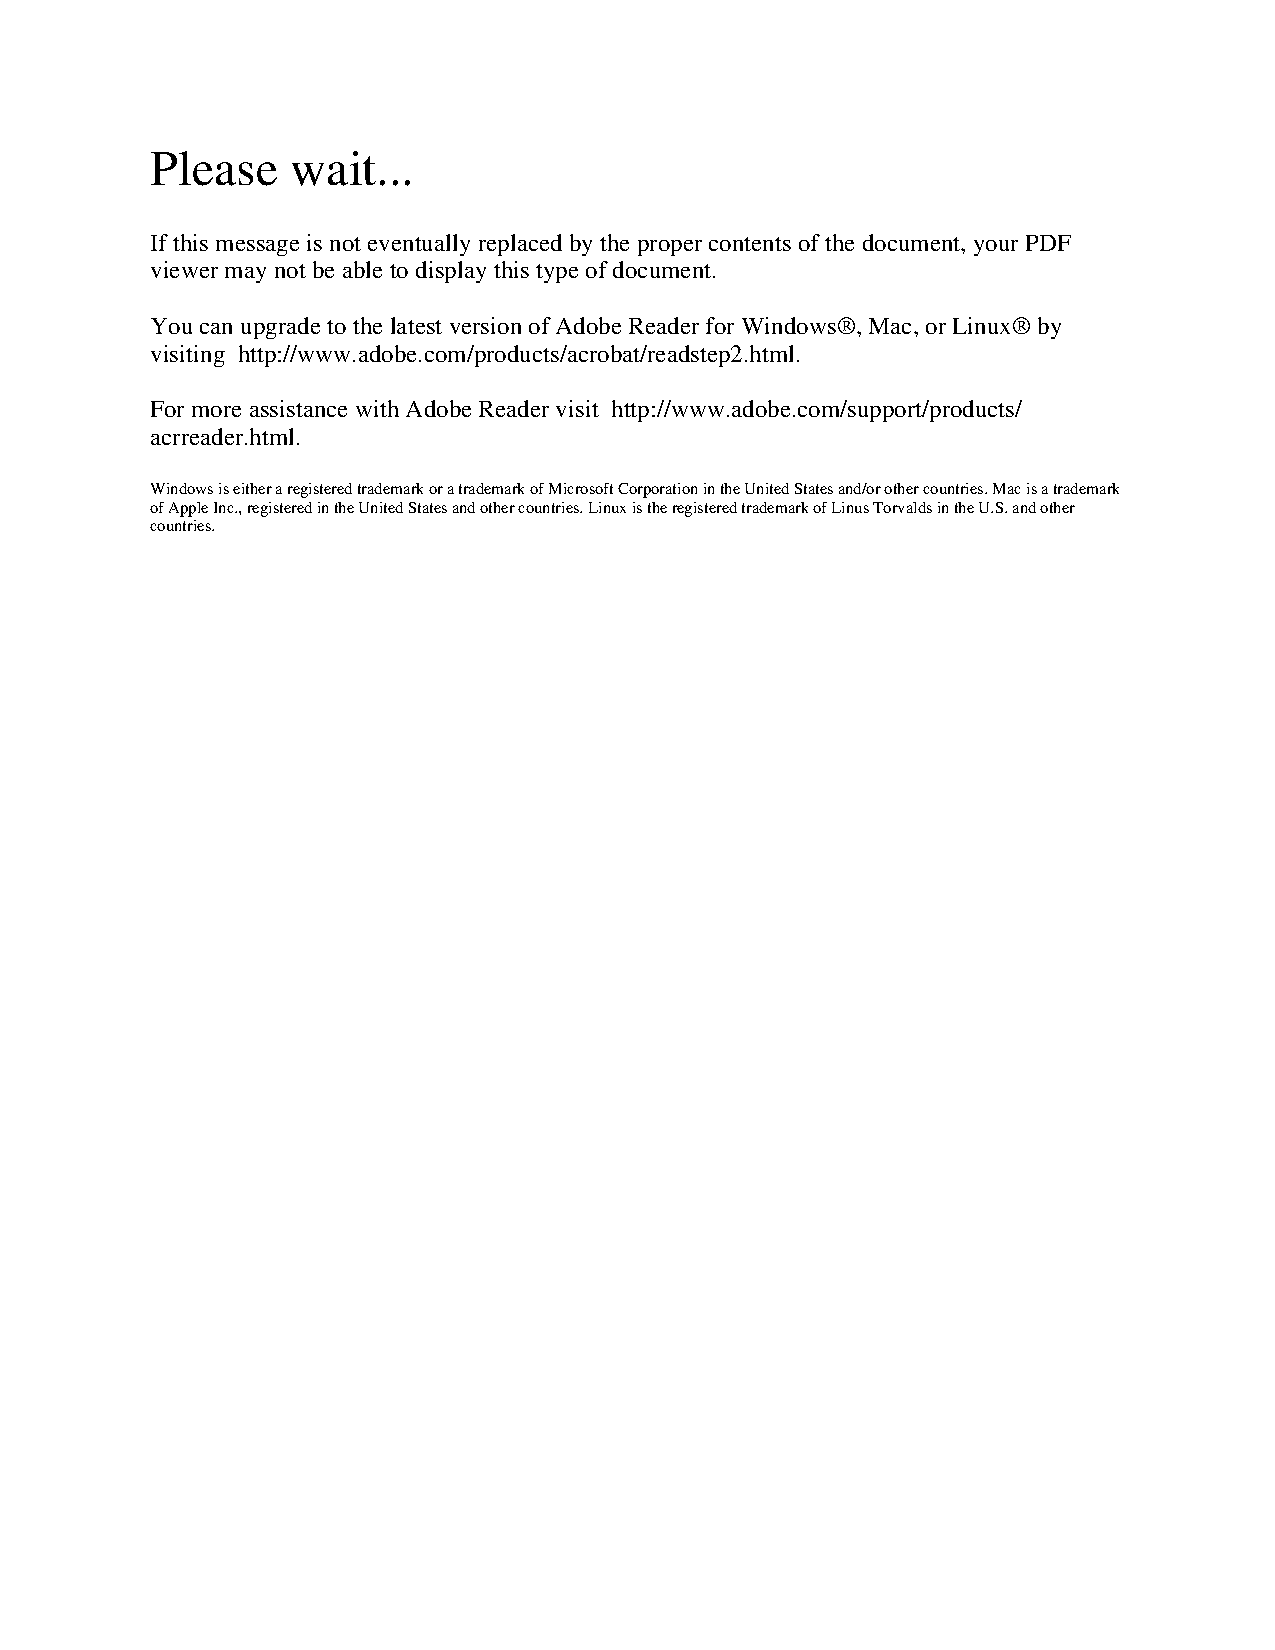
\includegraphics{confirmation.pdf}

% IMPORTANT
% you MUST include the ETH declaration of originality here; it is available for download on the course website or at http://www.ethz.ch/faculty/exams/plagiarism/index_EN; it can be printed as pdf and should be filled out in handwriting


%%%%%%%%%% Table of content %%%%%%%%%%%%%%%%%

\tableofcontents

\newpage

%%%%%%%%%%%%%%%%%%%%%%%%%%%%%%%%%%%%%%%

\renewcommand{\lstlistlistingname}{Matlabcode}
\lstlistoflistings
\cite{lamport94}

\listoffigures 
 \listoftables
\newpage
\fancyfoot[LE,RO]{Page\ \thepage}
\pagenumbering{arabic}

\section{Abstract}

\section{Individual contributions}

\subsection{Andermatt Samuel}
\begin{itemize}
\item Make the program object orientated
\item Implement the "Players from Literature"
\end{itemize}

\subsection{B\"osser Jonathan}
\begin{itemize}
\item Explore and explain GitHub [www.github.com]
\end{itemize}

\subsection{Meier David}
\begin{itemize}
\item Write the first version of the programm
\item Develop and implement "Tit for Average tat"
\end{itemize}

\section{Introduction and Motivations}
\subsection{The Prisoner's Dilema}
The prisoner's dilema is a model from game theory. 2 people are suspected to have done a crime together. Now they are examined seperatly in differnt rooms. In this situation, they can either whistle-blowing the other person to protect oneself or keep silent. Over all, it is of advantage, if both keep silent. But for the single person it is better to betray the other person. The risk of betraying is the following: if both accaused people betray the other, the penalty for both is the highest. This problem is in gametheory called "Prisoner's dilema"[Quelle: http://plato.stanford.edu/entries/prisoner-dilemma].

\subsection{The Axelrod Experiment}
In the year 1981, Robert Axelrod invited for a competition to the iterated prisoner's dilemma. People from different fields like mathematics, politics, economy or psychology have been asked to develop a winning strategy for this competition. All the different strategies were playing against another to find the most sucsessive strategy. Interesstingly, the very simple strategy "Tit for Tat" (TFT) won the tournament. During the first round, TFT keeps silent (cooperation) and during the rest of the game, just does, what its counterplayer did the round before.
This sort of experiment is very interessting, because the results can be applied in many different fields in real life. Just one out of many examples: 2 countries make an agreement on their amount of weapons. For the single country it is of advantage to haves more wmilitary strenth than the other nation. But as in the prisoner's dilema, if both nations rise their military strenth, for both it is just a loss money and an increase in danger.
[Quelle: Buch: Axelrod R. "Die Evolution der Kooperation" etc... (Google-Books)]

\subsection{Introduction of Noise}
A further development in the Axelrod Experiment is the introduction of noise. This means, cooperation is wrongly understood as defection and vise versa. The introduction of noise to the axelrod experiment ist nothing new[Quelle!!]. 

\section{Description of the Model and Players}

\subsection{Simple Players}
\subsubsection{Cooperative Player}
The player 1 is a very simple player: He always cooperates. This "decision" does not depend on any circumstances like the decisions of its antagonist. 

\subsubsection{Defective Player}
Also the player 2 is a very simple player: He always defects. 

\subsubsection{Random Player}
Like all players from this subsection, the decision of the random player does not depend on the results of the previous tournaments. The decision is randomly distributed and no decision is preferred.

\subsection{Players from Literatur}

All players in this subsection are taken from the first Axelrod's Turnament and implemented by us. Source: Lecture "Game Theory" [Quelle, Zitierung?!?]

\subsubsection{Tit for Tat}
The Player 4 during to the Axelrod Turnament the most successive player of all[Quelle]. The decision is the decision of the counterplayer from the last tournament. In the first round, the decision is cooperation. If the counter player cooperated during the last round, this player will cooperate in the current round.
www.socio.ethz.ch/vlib/pesb/pesb9.pdf

\subsubsection{Friedmann}
The Player "Friedmann" cooperates until its counter player defects once. After that, Friedmann now deflects for the rest of the game. This corresponds to "everlasting death".

\subsubsection{Pavlov}
Pavlov changes its decision every time when the counter player defects. But if the counter player cooperates, Pavlov gives the same decision as in the round before. The first decision is cooperation. 

\subsubsection{Tit for two Tat}
The first decision is cooperation. If the counter player cooperates, Tit for 2Tat" cooperates as well. Tit for 2 Tat only defects, if the counter player defected the last 2 rounds.

\subsubsection{Joss}
This is basically the same player like the player "Tit for Tat". The only difference: 10\% of the cooperative decisions are randomly defected.
www.socio.ethz.ch/vlib/pesb/pesb9.pdf

\subsubsection{Diekmann}
The player "Diekmann" plays basically Tit for Tat. The difference is, that every 10th move, he playes cooperative twice.
www.socio.ethz.ch/vlib/pesb/pesb9.pdf

\subsection{Own Players}

\subsubsection{Tit for Average Tat}
Based on the idea "Tit for Tat", we developed a player who averages the decisions of its opppnent over the last 5 Rounds. The first 5 rounds he plays Tit for Tat. To get a more forgiving player, he starts playing Tit for tat for 5 rounds.

\subsubsection{}

\section{Implementation}
In the following table 1 is shown the payoff matrix applied in our program.

\begin{table}


 \begin{center}
\begin{tabular}{|l|c|c|}
	  
\hline
   & Player B cooperates & Player B defects \\
  \hline
  Player A cooperates & A:3  B:3 & A:0  B:5  \\
 \hline
  Player A defects & A:5  B:0 &A:1 B:1 \\
 \hline
\end{tabular}
 \end{center}
 \caption{Reward Matrix}
\end{table}

Payoff matrix
Spielablauf
Informationen, die die Spieler sehen könnten
Art des Noises

\section{Simulation Results and Discussion}
Alle erfolgreichen Spieler spielen irgend auf eine art und weise tit for tat. Naja, trozdem evt. erwähnen, drauf eingehen

\section{Summary and Outlook}




\section{References}

\footnotesize
 \begin{thebibliography}{99}

\bibitem{HB98} Huynen, M.~A. and Bork, P. 1998. Measuring genome evolution. {\em
Proceedings of the National Academy of Sciences USA}
  95:5849--5856.

\bibitem{CA} Caprara, A. 1997. Sorting by reversals is difficult. In: {\em
Proceedings of the First Annual International Conference on Computational
Molecular Biology (RECOMB 97),} New York: ACM.  pp. 75-83.

\bibitem{MSW00}McLysaght, A., Seoighe, C. and Wolfe, K.~H. 2000. High frequency
of inversions during eukaryote gene order evolution.     In Sankoff, D. and
Nadeau, J.~H., editors, {\em Comparative Genomics},  Dordrecht, NL: Kluwer
Academic Press. pp. 47--58.

\bibitem{Rei91} Reinelt, G. 1991. {\em The Traveling Salesman - Computational
Solutions for TSP Applications.} Berlin: Springer Verlag.

\end{thebibliography}





Buch: Axelrod R. "Die Evolution der Kooperation", deutsche Fassung 2000

\appendix
\section{Submitted Researchplan}
\subsection{General Introduction}
Tournament like simulation of the prisoner's dilemma with repeated inter-
actions. Random errors are introduced in the information about the player's 
recent behavior. We want to observe the different outcome of the traditional
players if noise is introduced. Further we want to try to implement new 
players with learning strategies. \\
We believe that this makes the simulation more realistic.\\
Extension of Axelrod's Tournaments.

\subsection{Fundamental Questions}
Can a dispute based on miscommunication be overcome?\\
Can treason be hidden behind pretended miscommunication?\\
Does miscommunication discourage cooperation?\\
How much miscommunication can cooperation survive?\\
Do learning strategies have an advantage over the other ones?\\
How do the traditional players act and how does the final result change, 
if noise is introduced?\\
Independent variables: length of simulation, reliability of communication, rewards\\
Dependent variables: correlation between cooperation and success, frequency of cooperation, successful strategies

\subsection{Expected Results}
Miscommunication works against cooperating strategies.\\ 
Programs that reconcile are more successful.\\
The reward of the learning players is less influenced by the noise.

\subsection{References}

\begin{itemize}
\item On Evolving Robust Strategies for Iterated Prisoner's Dilemma, P. J. DARWEN and X. YAO, 16. November 1993\\
\item Multiagent Reinforcement Learning in the Iterated Prisoner's Dilemma, T. W. SANDHOLM and R. H. CRITES\\
\item Adaptation of Iterated Prisoner's Dilemma Strategies by Evolution and Learning, H. Y. QUEK and C. K. GOH, 2007\\
\item How to Cope with Noise in the Iterated Prisoner's Dilemma, J. WU and R. AXELROD, JOURNAL OF CONFLIC RTESOLUTION, Vol. 39 No. 1, March1995 183-189\\
\item Five Rules for the Evolution of Cooperation, M. A. NOWAK, Science 314, 1560 (2006)\\
\end{itemize}
\subsubsection{Research Methods}

Agent-Based Model

\subsection{Other}
The type(s) of the learning strategies we will decide later, after reading some of the literature.

\clearpage

\section{Matlabcode}

\subsection{Master.m}

\matlabscript{../matlab/Master}{Master.m}

\subsection{win.m}

\matlabscript{../matlab/win}{win.m}

\subsection{show\underline\ data.m}

\matlabscript{../matlab/show_data}{show\underline\ data.m}

\subsection{playerlist.m}

\matlabscript{../matlab/playerlist}{playerlist.m}

\subsection{player1.m}

\matlabscript{../matlab/player1}{player1.m}

\subsection{player2.m}

\matlabscript{../matlab/player2}{player2.m}

\subsection{player3.m}

\matlabscript{../matlab/player3}{player3.m}

\subsection{player4.m}

\matlabscript{../matlab/player4}{player4.m}

\subsection{player5.m}

\matlabscript{../matlab/player5}{player5.m}

\subsection{player6.m}

\matlabscript{../matlab/player6}{player6.m}

\subsection{player7.m}

\matlabscript{../matlab/player7}{player7.m}

\subsection{player8.m}

\matlabscript{../matlab/player8}{player8.m}

\subsection{player9.m}

\matlabscript{../matlab/player9}{player9.m}

\subsection{player10.m}

\matlabscript{../matlab/player10}{player10.m}

\subsection{player11.m}

\matlabscript{../matlab/player11}{player11.m}

\subsection{player12.m}

\matlabscript{../matlab/player12}{player12.m}

\subsection{player13.m}

\matlabscript{../matlab/player13}{player13.m}

\subsection{player14.m}

\matlabscript{../matlab/player14}{player14.m}

\subsection{player15.m}

\matlabscript{../matlab/player15}{player15.m}

\subsection{player16.m}

\matlabscript{../matlab/player16}{player16.m}

\subsection{player17.m}

\matlabscript{../matlab/player17}{player17.m}

\subsection{player18.m}

\matlabscript{../matlab/player18}{player18.m}

\subsection{player19.m}

\matlabscript{../matlab/player19}{player19.m}

\subsection{player20.m}

\matlabscript{../matlab/player20}{player20.m}








\end{document}  